\chapter{Overview}

\section{The Mobile Industry in Numbers}
Mobile penetration is approaching saturation in most markets around the world, especially among adult and urban populations. In every region, the majority of new subscribers will be young consumers and rural dwellers.
Despite increasing saturation in developed regions, there is still room for growth in many large, underpenetrated markets in developing regions. For example, India and Sub-Saharan Africa will account for around half of new mobile subscribers globally over the 2022–2030 period
“Globally, there were 4.4 billion mobile internet users in 2022, equivalent to 55% penetration”
The mobile internet usage gap has narrowed markedly in the last five years - from 50\% in 2017 to 41\% in 2022 on average – as more people around the world rely on the internet for many daily activities, especially in the wake of the Covid-19 pandemic. 
\subsection{5G in The Mobile Market}
“5G will overtake 4G in 2029 to become the dominant mobile technology by the end of this decade”
5G adoption continues to rise due to new network deployments and cheaper devices. As of January 2023, there were 229 commercial 5G networks around the world and over 700 5G smartphone models had been launched, including more than 200 in 2022. 
The number of connections on legacy networks (2G and 3G) will continue to decline in the coming years as users migrate to 4G and 5G, resulting in more network shutdowns. To date, operators have announced plans to shut down 96 2G networks and 107 3G networks around the world.

\begin{figure}[h]
\centering
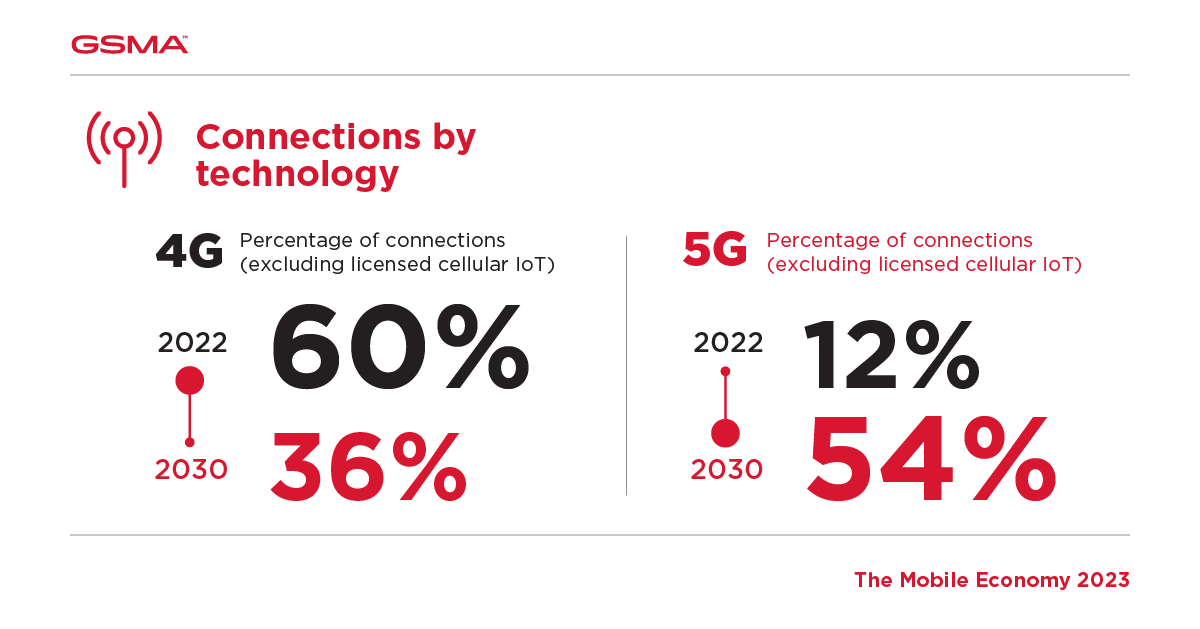
\includegraphics[width=3.54 in, height=1.85in]{1.PNG}
\caption{4G vs 5G connections }
\label{fig:figure1.1}
\end{figure}


\section{The Next Generation - 5G NR}
Despite LTE being a very capable technology, there are requirements not possible to meet with LTE or its evolution. Furthermore, technology development over the more than 10 years that have passed since the work on LTE was initiated allows for more advanced technical solutions. To meet these requirements and to exploit the potential of new technologies, 3GPP initiated the development of a new radio access technology known as NR (New Radio). A workshop setting the scope was held in the fall of 2015 and technical work began in the spring of 2016. The first version of the NR specifications was available by the end of 2017 to meet commercial requirements on early 5G deployments already in 2018.
NR reuses many of the structures and features of LTE. However, being a new radio-access technology means that NR, unlike the LTE evolution, is not restricted by a need to retain backwards compatibility. The requirements on NR are also broader than what was the case for LTE, motivating a partly different set of technical solutions.

\subsection{5G Use Cases}
In the context of 5G, one is often talking about three distinctive classes of use cases: enhanced mobile broadband (eMBB), massive machine-type communication (mMTC), and ultra-reliable and low-latency communication (URLLC) 
\begin{itemize}
    \item eMBB corresponds to a more or less straight forward evolution of the mobile broadband services of today, enabling even larger data volumes and further enhanced user experience, for example, by supporting even higher end-user data rates.
    \item mMTC corresponds to services that are characterized by a massive number of devices, for example, remote sensors, actuators, and monitoring of various equipment. Key requirements for such services include very low device cost and very low device energy consumption, allowing for very long device battery life of up to at least several years. Typically, each device consumes and generates only a relatively small amount of data, that is, support for high data rates is of less importance.
    \item URLLC type-of-services are envisioned to require very low latency and extremely high reliability. Examples hereof are traffic safety, automatic control, and factory automation. 
\end{itemize}
It is important to understand that the classification of 5G use cases into these three distinctive classes is somewhat artificial, primarily aiming to simplify the definition of requirements for the technology specification. There will be many use cases that do not fit exactly into one of these classes. Just as an example, there may be services that require very high reliability but for which the latency requirements are not that critical. Similarly, there may be use cases requiring devices of very low cost but where the possibility for very long device battery life may be less important.

\begin{figure}[h]
\centering
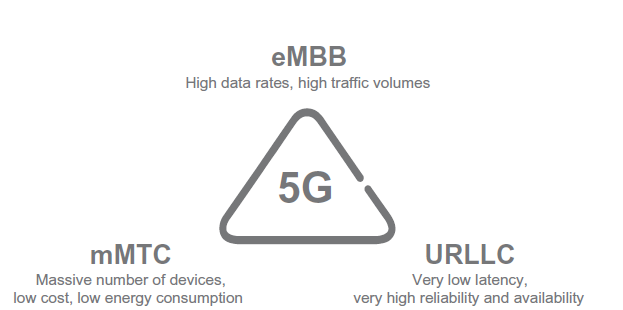
\includegraphics[width=4.76in, height=2.37in]{2.PNG}
\caption{5G Use cases classification}
\end{figure}

\subsection{Waveform, Numerology, and Frame Structure}

The choice of radio waveform is the core physical layer decision for any wireless access technology. After assessments of all the waveform proposals, 3GPP agreed to adopt orthogonal frequency division multiplexing (OFDM) with a cyclic-prefix (CP) for both DL and UL transmissions. CP-OFDM can enable low implementation complexity and low cost for wide bandwidth operations and multiple-input multiple-output (MIMO) technologies. 
NR supports operation in the spectrum ranging from sub-1 GHz to millimeter wave bands. Two frequency ranges (FR) are defined in Release 15:
\begin{itemize}
    \item FR1: 450 MHz – 6 GHz, commonly referred to as sub-6 GHz.
    \item FR2: 24.25 GHz – 52.6 GHz, commonly referred to as millimeter wave. 
\end{itemize}
	 
	  

Scalable numerologies are key to support NR deployment in such a wide range of spectrum. NR adopts flexible sub-carrier spacing of $2^\alpha \times 15$ kHz $(\alpha = 0,1,...,4 )$  scaled from the basic 15 kHz sub-carrier spacing in LTE. Accordingly, the CP is scaled down by a factor of $2^\alpha$ from the LTE CP length of 4.7 $\mu$s. This scalable design allows support for a wide range of deployment scenarios and carrier frequencies. At lower frequencies, below 6 GHz, cells can be larger and sub-carrier spacings of 15 kHz and 30 kHz are suitable. At higher frequencies, cells and delay spread are typically smaller and the CP lengths provided by the 60 and 120 kHz numerologies are sufficient.

A frame has a duration of 10ms and consists of 10 subframes. This is the same as in LTE, facilitating NR and LTE coexistence. Each subframe consists of $2^\alpha$ slots of 14 OFDM symbols each. Although a slot is a typical unit for transmission upon which scheduling operates, NR enables transmission to start at any OFDM symbol and last only as many symbols as needed for the communication. This type of “mini-slot” transmission can thus facilitate very low latency for critical data as well as minimize interference to other links per the lean carrier design principle that aims at minimizing transmissions. Latency optimization has been an important consideration in NR. Many other tools besides “mini-slot” transmission have been introduced in NR to reduce latency.
\begin{figure}[h]
\centering
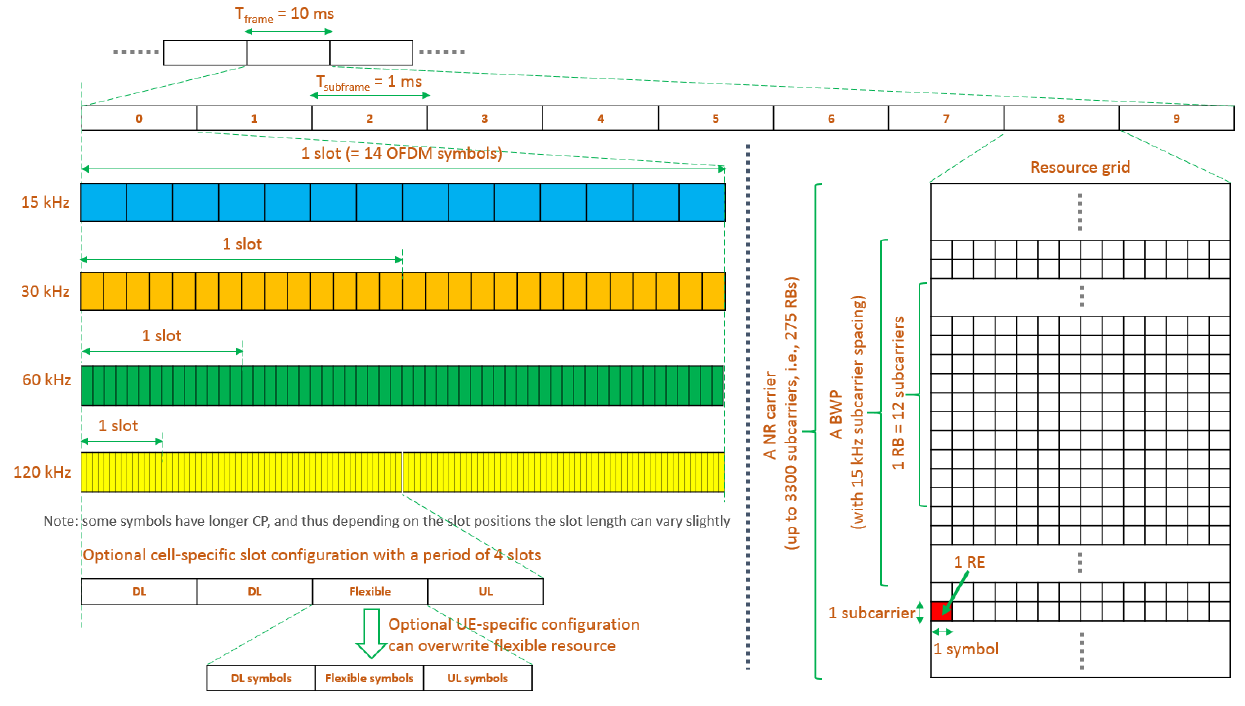
\includegraphics[width=6in, height=3.4in]{3.PNG}
\caption{5G Frame structure}
\end{figure}

\section{5G Data Channels: Logical, Transport \& Physical}

In order to be able to carry the data across the 5G radio access network, the data and information is organized into a number of data channels.
By organizing the data into various channels the 5G communications system is able to manage the data transfers in an orderly fashion and the system is able to understand what data is arriving and hence it is able to process it in the required fashion.
As there are many different types of data that need to be transferred - user data obviously needs to be transferred, but so does control information to manage the radio communications link, as well as data to provide synchronization, access and the like. All of these functions are essential and require the transfer of data over the radio access network. The 5G mobile or wireless communications system uses a similar access stratum to that used by 4G LTE.
Although there are two protocol stacks: user plane and control plane, they still adopt the familiar OSI reference model.
As a result there are various protocol layers and accordingly there are several data channel layers that are defined for the radio communications.
In order to group the data to be sent over the 5G NR radio access network, the data is organised in a very logical way. As there are many different functions for the date being sent over the radio communications link, they need to be clearly marked and have defined positions and formats.To ensure this happens, there are several different forms of data "channel" that are used. The higher level ones are "mapped" or contained within others until finally at the physical level, the channel contains data from higher level channels.
In this way there is a logical and manageable flow of data from the higher levels of the protocol stack down to the physical layer.
There are three main types of data channels that are used within mobile communications systems. This is true for 5G systems, and accordingly the hierarchy is given below.
\begin{itemize}
    \item Logical channel: Logical channels can be one of two groups: control channels and traffic channels:
    \begin{itemize}
        \item Control channels: The control channels are used for the transfer of data from the control plane
        \item Traffic channels: The traffic logical channels are used for the transfer of user plane data.
    \end{itemize}
    \item Transport channel: Is the multiplexing of the logical data to be transported by the physical layer and its channels over the radio interface.
    \item Physical channel : The physical channels are those which are closest to the actual tr-ansmission of the data over the radio access network / 5G RF signal. They are used to carry the data over the radio interface.
\end{itemize}
The physical channels often have higher level channels mapped onto them of provide a specific service. Additionally, the physical channels carry payload data or details of specific data transmission characteristics like modulation, reference signal multiplexing, transmit power, RF resources, etc.

\subsection{5G NR logical channels}
There are several different logical channels that are used within the 5G NR radio access network. Some of them will be familiar names from the 4G LTE system as the names have been carried over.
\begin{itemize}
    \item \textbf{Broadcast Control Channel (BCCH)}: The BCCH is used within the downlink, and it is used for sending broadcast style information to the UE within that cell. The system information transmitted by the 5G NR BCCH is divided into different blocks:
    \begin{itemize}
        \item Master Information Block (MIB): There is one MIB and this is mapped onto the BCH transport channel and then to the PBCH physical channel.
        \item System Information Block (SIB): There are several system information blocks, SIBs. These are mapped onto the DL-SCH transport channel and then onto the PDSCH physical channel.
    \end{itemize}
    \item \textbf{Paging Control Channel (PCCH)}: This is a Downlink channel. It is used to page the UEs whose location at cell level is not known to the network. As a result the paging message needs to be transmitted in multiple cells. The PCCH is mapped to the PCH transport channel and then to the PDSCH physical channel.
    \item \textbf{Common Control Channel (CCCH)}: This 5G channel is used on both the downlink and uplink for transmitting control information to and from the user equipments or mobiles. The channel is used for initial access, i.e. those mobiles that do not have a radio resource control, RRC connection.
    \item \textbf{Dedicated Control Channel (DCCH)}: The DCCH is used within the uplink and downlink to carry dedicated control information between the UE or mobile and the network. It is used by the UE and the network after a radio resource control, RRC connection has been established.
    \item \textbf{Dedicated Traffic Channel (DTCH)}: This 5G channel is present in both the uplink and downlink. It is dedicated to one UE and is used for carrying user information to and from a specific UE and the network.
\end{itemize}

\subsection{5G NR transport channels}
There are \emph{five different transport channels.} Some are used on the uplink, others on the downlink, and some can be used on both.

\begin{itemize}
    \item \textbf{Broadcast Channel (BCH)}: The BCH 5G channel is used in the downlink only for transmitting the BCCH system information and specifically the Master Information Block, MIB, information. In order that the data can be utilized, it has a specific format.
    \item \textbf{Paging Channel (PCH)}: The PCH is used for carrying paging information from the PCCH logical channel. The PCH supports discontinuous reception, DRX, to enable the UE to save battery power by waking up at a specific time to receive the PCH.
    \newline
    In order that the PCH is received by all mobiles / UEs in the cell, the PCH must be broadcast over the entire cell as a single message, or where beam forming is used, this can be done using several different PCH instances.
    \item \textbf{Downlink Shared Channel (DL-SCH)}: As the name indicates, this is a downlink only channel. It is the main transport channel used for transmitting downlink data and it supports all the key 5G NR features. These include: dynamic rate adaptation; HARQ, channel aware scheduling, and spatial multiplexing.
    \newline
    The DL-SCH is also used for transmitting some parts of the BCCH system information, specifically the SIB. Each UE has a DL-SCH for each cell it is connected to.
    \item \textbf{Uplink Shared Channel (UL-SCH)}: This is the uplink counterpart to the DLSCH that is, the uplink transport channel used for transmission of uplink data.
    \item \textbf{Random-Access Channel (RACH)}: The RACH is a transport channel, which carries the random access preamble which is used to overcome the message collisions that can occur when UEs access the system simultaneously.
\end{itemize}

\subsection{5G NR physical channels}
The 5G physical channels are used to transport information over the actual radio interface. They have the transport channels mapped into them, but they also include various physical layer data required for the maintenance and optimization of the radio communications link between the UE and the base station.
The 5G mobile communications physical layer channels resemble those of 4G LTE, but PHICH and PCIICH have been removed. The HARQ operation has also been updated to be more flexible. Also the downlink control channel PDCCH is now administered by layer 3 procedures.
There are \emph{three physical channels} for each of the uplink and downlink

\subsubsection{5G NR Downlink Physical Channels}
\begin{description}
    \item[Physical downlink shared channel (PDSCH):] 5G NR physical downlink shared channel, PDSCH carries data sharing the capacity on a time and frequency basis. The PDSCH physical channel carries a variety of items of data: user data; UE-specific higher layer control messages mapped down from higher channels; system information blocks (SIBs) \& paging. \\
    The PDSCH uses an adaptive modulation format dependent upon the link conditions, i.e. signal to noise ratio. It also uses a flexible coding scheme. The combination of these means that there is a flexible coding and data rate.
    \item[Physical downlink control channel (PDCCH):] As the name implies, 5G physical downlink control channel carries downlink control data. Its primary function is scheduling the downlink transmissions on the PDSCH and also the uplink data transmissions on the PUSCH.\\
    The PDCCH uses QPSK as its modulation format and polar coding as the coding scheme, except for small packets of data.
    \item[Physical broadcast channel (PBCH):] This 5G channel forms part of the synchronization signal block. Its function is to provide UEs with the Master Information Block, MIB. A further function of the PBCH in conjunction with the control channel is to support the synchronization of time and frequency. This aids with cell acquisition, selection and re-selection.\\
    The PBCH uses a fixed data format and there is one block that extends over a TTI of 80ms, uses QPSK modulation and it transmits a cell specific demodulation reference signal, DMRS pattern that can be used aid with beam-forming.
\end{description}

\subsubsection{5G NR Uplink Physical Channels}
\begin{description}
    \item[Physical random access channel (PRACH):] This 5G channel is used for channel access. It transmits an initial random access pre-amble consisting of sequences which may be of two different lengths:
    \begin{itemize}
        \item A long sequence is 839 which is applied to the subcarrier spacings of 1.25kHz and 5 kHz
        \item Short sequence lengths of 139 are applied to subcarrier spacings of 15 kHz and 30 kHz (FR1 bands) and 60 kHz and 120 kHz (FR2 bands).
    \end{itemize}
    
    \item[Physical uplink shared channel (PUSCH):] The counterpart of the PDSCH. It is used to carry data from the UL-SCH and its higher mapped channels on a frequency and time-shared basis.\\
    Like the PDSCH, The PUSCH also has a very flexible format. The allocation of frequency resources is undertaken using resource blocks along with a flexible modulation and coding scheme dependent upon the link signal to noise ratio.\\
    To support the channel link estimation and demodulation, the PUSCH contains DMRS signals.
    \item[Physical uplink control channel (PUCCH):] This carries the uplink control data. It is also possible that dependent upon the resource allocation the uplink control information or data may also be sent on the PUSCH, even though in the downlink direction, control information is always sent on the PDCCH.
\end{description}
	
The use of these 5G channels provide a method for organizing the flow of data over the radio interface of the 5G communications network. Using channels enables the communications system to recognize the type of data that is being sent, and to deal with it accordingly. The format used is very similar to that employed on 4G LTE and it built on the technology of previous mobile communications or mobile phone generations.
\newline\newline
Figures \ref{fig:sub-first} \& \ref{fig:second} shows the mapping between logical, transport and physical channels in both DL and UL
\begin{figure}[h]
    \centering
    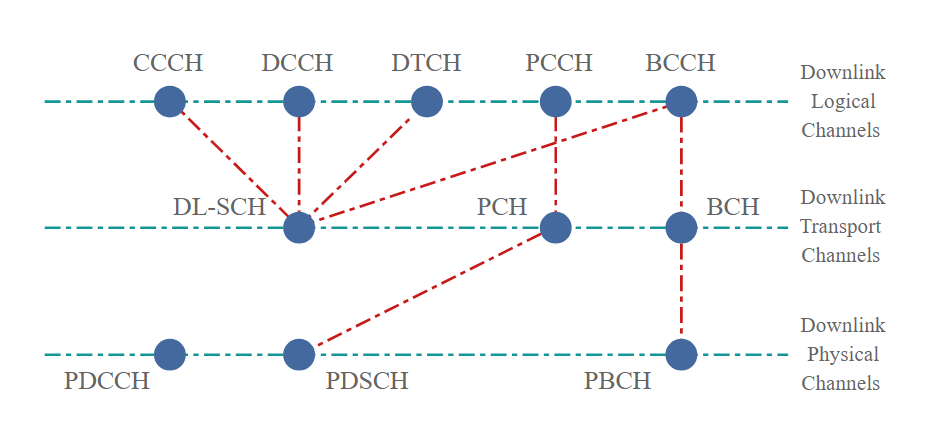
\includegraphics[width=4.31in, height = 2in]{4.PNG}
    \caption{5G Downlink logical, transport and physical channel mapping}
    \label{fig:sub-first}
\end{figure}

\begin{figure}[h]
    \centering
    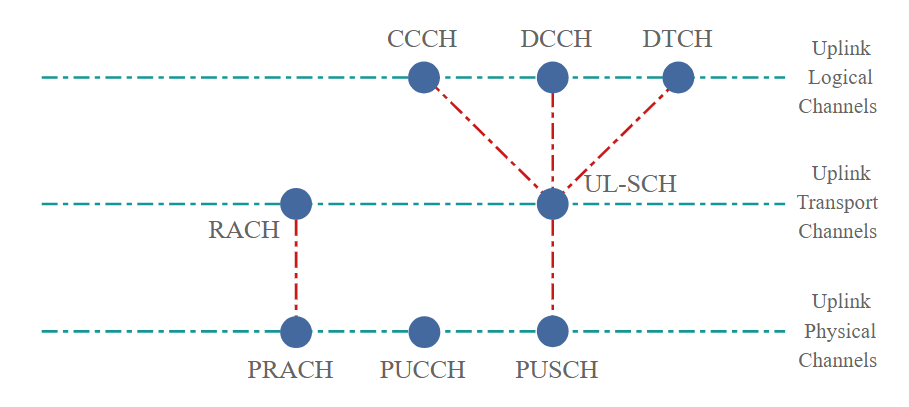
\includegraphics[width=4.31in, height = 2in]{5.PNG}
    \caption{5G Uplink logical, transport and physical channel mapping}
    \label{fig:second}
\end{figure}
